\section{Produção de ar comprimido}

\begin{frame}{Compressor}
	\begin{block}{Introdução}
		O \textit{compressor} é responsável por \textbf{pressurizar} o ar que será utilizado no sistema pneumático.
		
		Ele pode usar dois métodos para tal:
		\begin{itemize}
			\item \textbf{Compressor de deslocamento positivo}
			
			Reduz o volume do ar: o ar é admitido em uma câmara isolada do meio exterior, na qual o seu volume é gradualmente diminuído, processando-se a compressão.
			
			\item \textbf{Compressor de deslocamento dinâmico}
			
			Aumenta-se a quantidade de ar num mesmo volume: as lâminas do compressor empurram o ar dentro de um compartimento fechado, e um sistema de difusores retarda seu escoamento, gerando um aumento na pressão.
		\end{itemize}
	\end{block}
\end{frame}


\begin{frame}{Compressor}
\centering
\begin{tikzpicture}[xscale=1.5]
	\node (init) at (0,0) {Compressores};
	\node[coordinate] (m1) at (0,-0.5) {};
	
	\node (pos) at (-1.5,-1) {Deslocamento positivo};
	\node[coordinate] (m2pos) at (-1.5,-1.5) {};
	\node (din) at (1.5,-1) {Deslocamento dinâmico};
	\node[coordinate] (m2din) at (1.5,-1.5) {};
	
	\node (dinRad) at (2.25,-2) {Fluxo radial};
	\node (dinAx) at (0.75,-2) {Fluxo axial};
	\node (posRot) at (-2.25,-2) {Rotativos};
	\node (posAlt) at (-0.75,-2) {Alternativos};
	
	\draw ($ (posRot)+(-0.3,-0.2) $) -- ++(0,-0.5) node[right=5pt] 
	{Parafuso} -- ++(0,-0.5) node[right=5pt] {Palhetas};
	
	\draw[->] ($ (posRot)+(-0.3,-0.7) $) -- +(4pt,0);
	\draw[->] ($ (posRot)+(-0.3,-1.2) $) -- +(4pt,0);
	
	\draw ($ (posAlt)+(-0.3,-0.2) $) -- ++(0,-0.5) node[right=5pt] 
	{Pistão};
	
	\draw[->] ($ (posAlt)+(-0.3,-0.7) $) -- +(4pt,0);
	
	\draw (init) -- (m1) -| (din);
	\draw (init) -- (m1) -| (pos);
	
	\draw (din) -- (m2din) -| (dinRad);
	\draw (din) -- (m2din) -| (dinAx);
	\draw (pos) -- (m2pos) -| (posRot);
	\draw (pos) -- (m2pos) -| (posAlt);
\end{tikzpicture}
\end{frame}


\begin{frame}{Compressor de deslocamento positivo}
\begin{block}{Compressor rotativo de parafuso}
	\begin{itemize}
		\item Consiste em dois parafusos helicoidais, os quais, pelos perfis côncavo e convexo, comprimem gradualmente o ar, que é conduzido axialmente. No tubo de descarga o ar é descarregado continuamente e livre de pulsações.
	\end{itemize}
\end{block}

\begin{minipage}{0.45\linewidth}
	\centering
	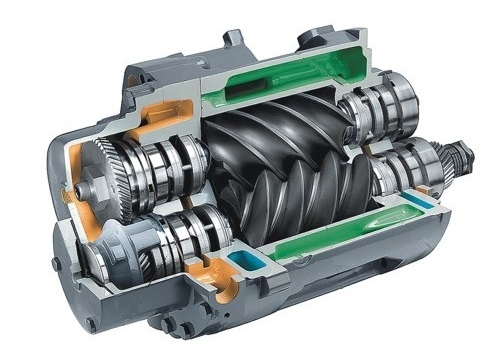
\includegraphics[width=1\linewidth]{Figuras/Ch12/fig1}
\end{minipage}
\hfill
\begin{minipage}{0.45\linewidth}
	\centering
	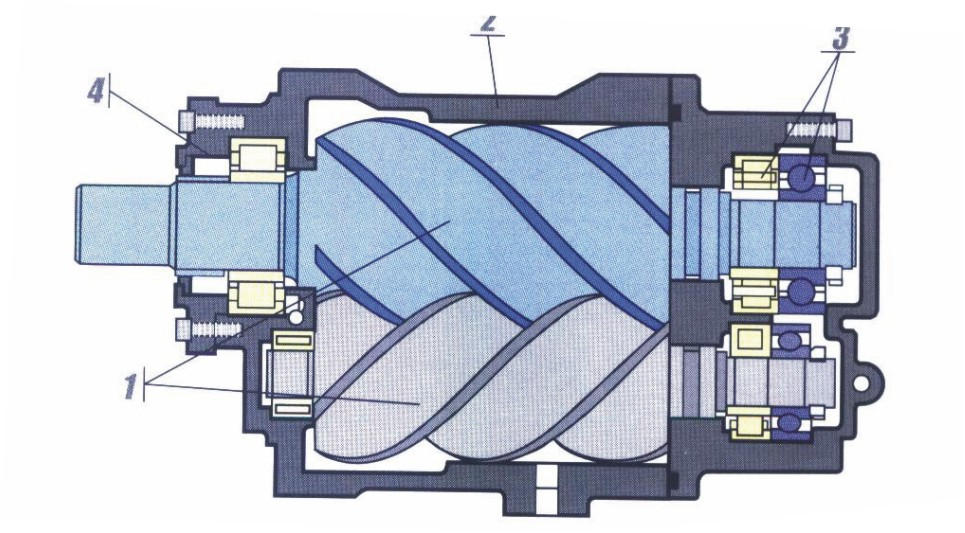
\includegraphics[width=1\linewidth]{Figuras/Ch12/fig1n2}
\end{minipage}
\end{frame}


\begin{frame}{Compressor de deslocamento positivo}
	\begin{block}{Compressor rotativo de palhetas}
		\begin{itemize}
			\item Consiste em um eixo excêntrico (posicionado fora do centro) com palhetas móveis. O ar percorre um caminho onde o volume é reduzido gradualmente.
		\end{itemize}
	\end{block}

	\vspace{0.5cm}
	
	\begin{minipage}{0.45\linewidth}
		\centering
		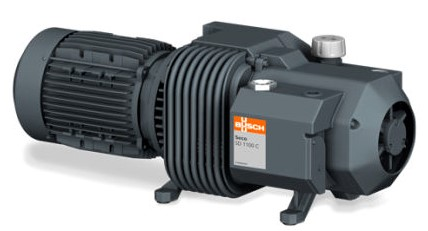
\includegraphics[width=1\linewidth]{Figuras/Ch12/fig2}
	\end{minipage}
	\hfill
	\begin{minipage}{0.45\linewidth}
		\centering
		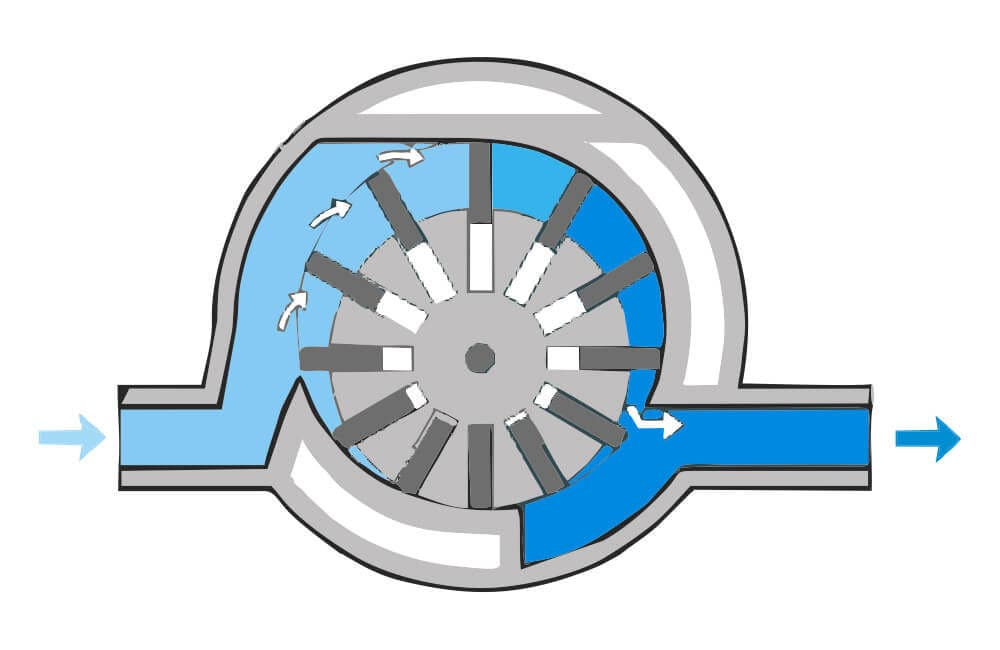
\includegraphics[width=1\linewidth]{Figuras/Ch12/fig3}
	\end{minipage}
\end{frame}


\begin{frame}{Compressor de deslocamento positivo}

\centering
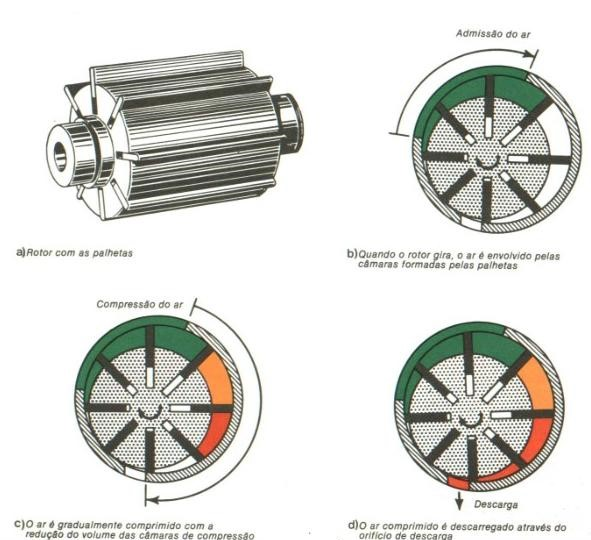
\includegraphics[width=0.6\linewidth]{Figuras/Ch12/fig3n2}

\medskip
Ciclo de operação de um compressor rotativo de palhetas
\end{frame}


\begin{frame}{Compressor de deslocamento positivo}
	\begin{block}{Compressor alternativo de pistão}
		\begin{itemize}
			\item Consiste em um compartimento com duas passagens (entrada/saída) e um pistão. Ora o pistão se contrai, reduzindo a pressão no compartimento e admitindo ar pela entrada e ora esse se estende, pressurizando o ar no compartimento que é então, liberado pela saída.
			\item É o compressor mais utilizado. Ele é apropriado para baixas, médias e também altas pressões.
		\end{itemize}
	\end{block}
	
%	\vspace{0.5cm}
	
	\begin{minipage}{0.45\linewidth}
		\centering
		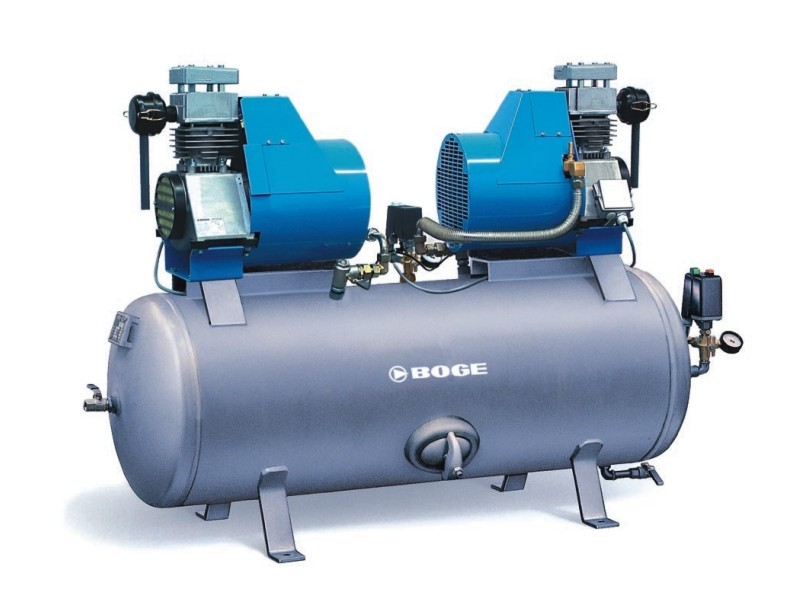
\includegraphics[width=1\linewidth]{Figuras/Ch12/fig4}
	\end{minipage}
	\hfill
	\begin{minipage}{0.45\linewidth}
		\centering
		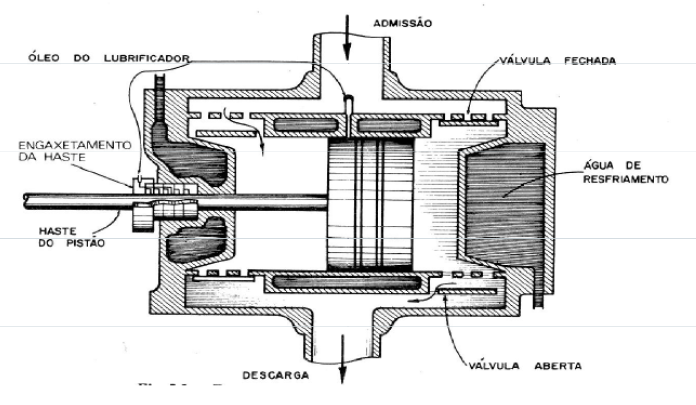
\includegraphics[width=1\linewidth]{Figuras/Ch12/fig5}
	\end{minipage}
\end{frame}


%o ar admitido é colocado em contato com impulsores (análogo às lâminas do ventilador da sua casa) em alta velocidade. Este ar é acelerado, ganhando energia cinética. Posteriormente, seu escoamento é retardado por meio de difusores, obrigando a uma elevação de pressão.


\begin{frame}{Compressor de deslocamento dinâmico}
	\begin{block}{Compressor de fluxo axial}
		\begin{itemize}
			\item Em geral, os compressores axiais são empregados em locais onde se requer um consumo relativamente elevado e constante.
		\end{itemize}
	\end{block}
	
	%	\vspace{0.5cm}
	
	\centering
	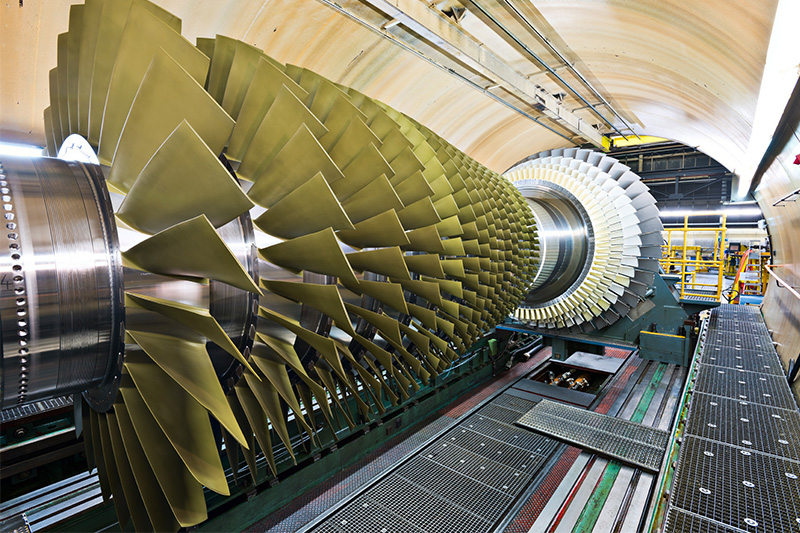
\includegraphics[width=0.7\linewidth]{Figuras/Ch12/fig6}
\end{frame}


\begin{frame}{Compressor de deslocamento dinâmico}
	\begin{block}{Compressor de fluxo radial}
		\begin{itemize}
			\item O ar é deslocado por uma ou mais hélices, onde a energia cinética é convertida em energia de pressão.
		\end{itemize}
	\end{block}
	
	%	\vspace{0.5cm}
	
	\centering
	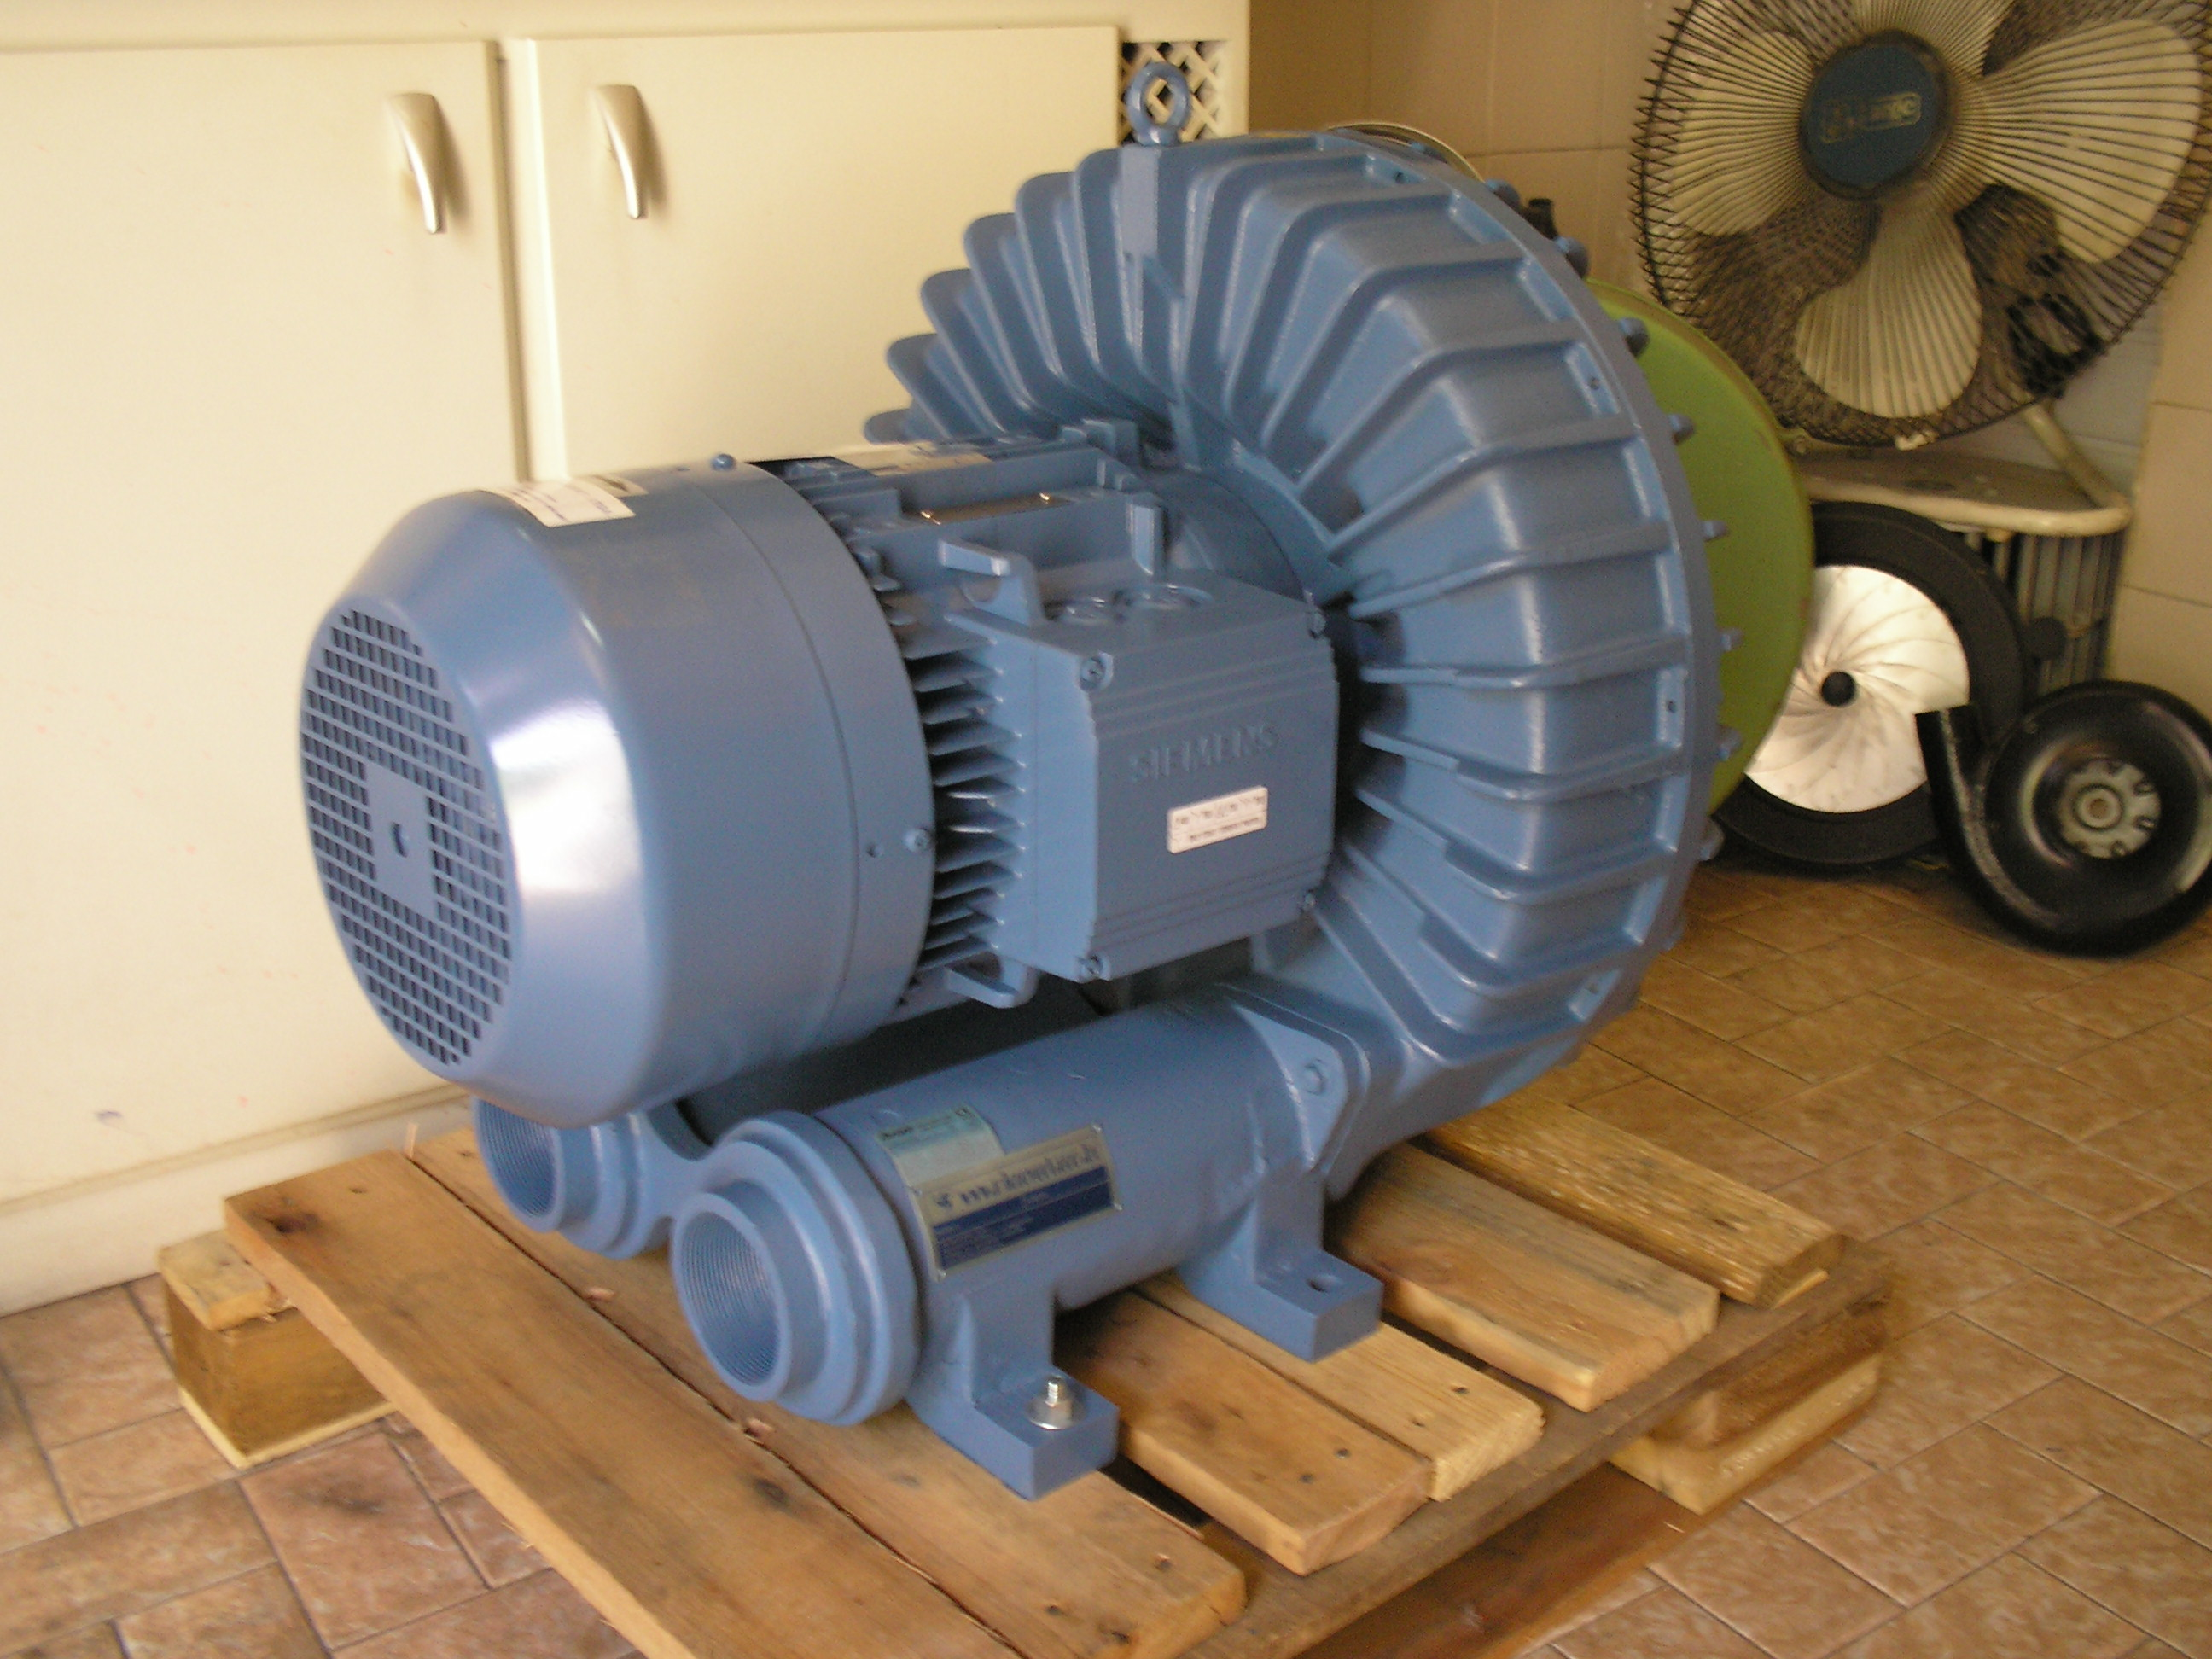
\includegraphics[width=0.65\linewidth]{Figuras/Ch12/fig7}
\end{frame}


\begin{frame}{Compressor}
	\begin{block}{Turbinas}
		\begin{itemize}
			\item As turbinas de avião são uma das aplicações de compressores de deslocamento dinâmico.
		\end{itemize}
	\end{block}
	
	\vspace{0.5cm}

	\centering
	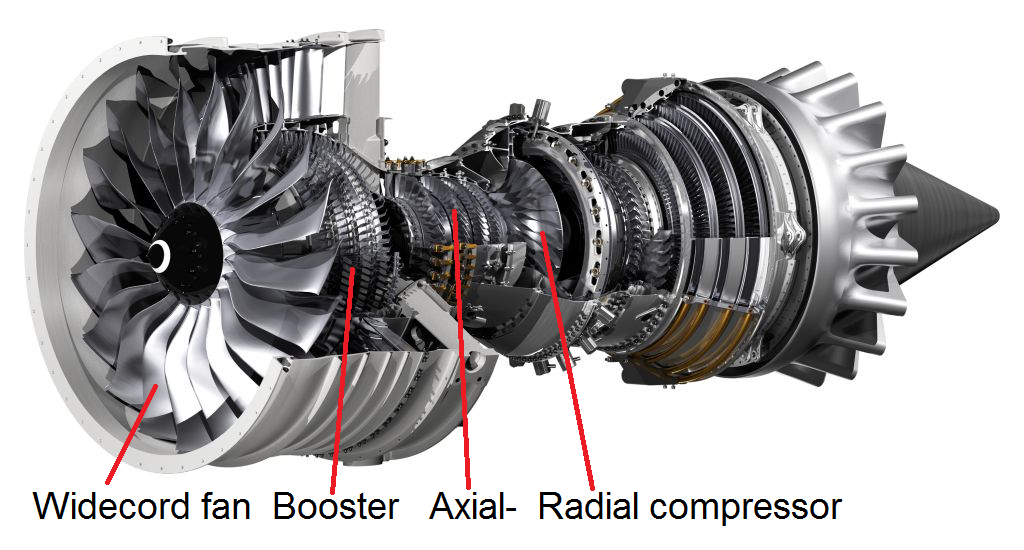
\includegraphics[width=0.8\linewidth]{Figuras/Ch12/fig9}

\end{frame}


\begin{frame}{Compressor}
	\centering
	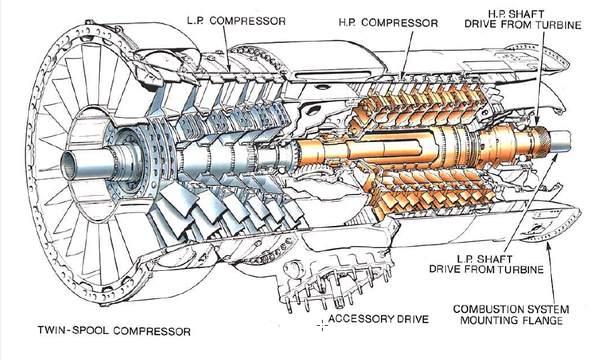
\includegraphics[width=1\linewidth]{Figuras/Ch12/fig8}

	Interior da turbina
\end{frame}


\begin{frame}{Sistema de refrigeração do compressor}
\begin{block}{Introdução}
	\begin{itemize}
		\item O processo de compressão é \textbf{exotérmico}, isto é, \textbf{gera calor}.
		\item O calor é gerado pois há \textbf{atrito entre as moléculas do fluido e as partes do compressor.}
		\item Compressores pequenos e médios são equipados com um \textbf{ventilador} acoplado na polia de transmissão para dissipar o calor.
		\item Compressores com uma potência de acionamento superior a \SI{30}{\kilo\watt}	(\SI{40}{\HP}), devem ser equipados com \textbf{refrigeração a água.}
	\end{itemize}
\end{block}
\end{frame}


\begin{frame}{Sistema de refrigeração do compressor}
	\begin{block}{Objetivos}
		\begin{itemize}
			\item Controlar a \textbf{temperatura} das válvulas, do óleo lubrificante e do ar que está sendo comprimido.
			\item Compressão \textbf{isotérmica} - dificultada pela falta de superfície para troca de calor.
			\item Evitar \textbf{deformação} dos componentes do compressor.
			\item Aumentar a \textbf{eficiência} do compressor.
		\end{itemize}
	\end{block}
\end{frame}


\begin{frame}{Sistema de refrigeração do compressor}
	\begin{block}{Resfriamento a água}
		\begin{itemize}
			\item Os blocos dos cilindros têm paredes duplas,	entre as quais circula água.
			\item A superfície que exige um melhor resfriamento é a do cabeçote, pois permanece em contato	com o ar comprimido ao fim da compressão. 
			\item O ar a ser resfriado passa em torno dos tubos, transferindo o calor para a água em circulação.
		\end{itemize}
	\end{block}

\centering
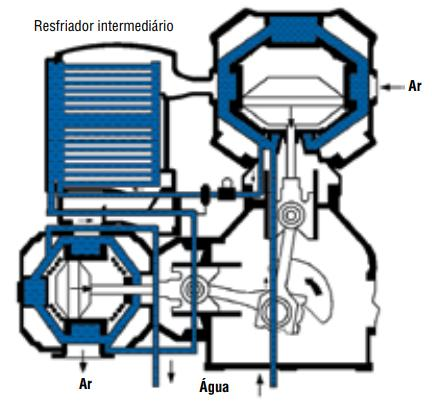
\includegraphics[height=0.5\textheight]{Figuras/Ch12/fig11n2}

\end{frame}


\begin{frame}{Sistema de refrigeração do compressor}
	\centering
	
\includegraphics[width=0.8\linewidth]{Figuras/Ch12/fig11}
	
	Resfriamento a água
\end{frame}


\begin{frame}{Sistema de refrigeração do compressor}
	\begin{block}{Resfriamento a ar}
		Existem dois modos básicos de resfriamento por ar:
		\begin{itemize}
			\item \textbf{Circulação}
			
			Os cilindros e cabeçotes, geralmente, são aletados a fim de
			proporcionar maior troca de calor, o que é feito por meio da
			circulação do ar ambiente e com auxílio de hélices nas polias de transmissão.
			
			\item \textbf{Ventilação forçada}
			
			A refrigeração interna dos cabeçotes e resfriador intermediário
			é conseguida através de ventilação forçada, ocasionada
			por uma ventoinha, obrigando o ar a circular no interior do
			compressor.
		\end{itemize}
	\end{block}
\end{frame}


\begin{frame}{Sistema de refrigeração do compressor}
	\centering
	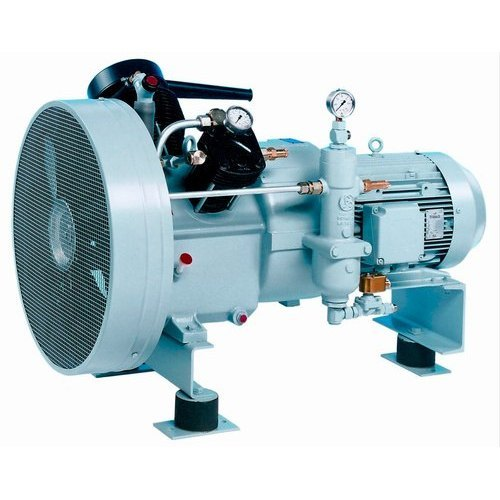
\includegraphics[width=0.6\linewidth]{Figuras/Ch12/fig10}
	
	Resfriamento a ar (ventilação forçada)
\end{frame}


\frame{
	\frametitle{Exercícios}
	\begin{block}{}
		01. Uma turbina de alto porte será instalada em um protótipo da Boeing para um cargueiro militar. Qual dos tipos de refrigerador intermediário você acha que deve ser usado? Por quê?
	\end{block}
}

\section*{Referências}
\frame{
	\frametitle{Referências e Exercícios Complementares}
	\begin{itemize}
		\item MELCONIAN, Sarkis. Sistemas Fluidomecânicos - Hidráulica e Pneumática, 1 ed. Érica, 2014.
	\end{itemize}
	%\centering{\alert{Página 546 - \textbf{Capítulo 6}}} \\
	%\centering{\alert{Lista de exercícios 01}}
}